\newacronym{ros}{ROS}{Robot Operating System}
\newacronym{dgps}{DGPS}{Differential Global Positioning System}
\newacronym{gnss}{GNSS}{Global Navigation Satellite System}
\newacronym{rtcm}{RTCM}{Radio Technical Commission for Maritime Services}

%-----------------------
\chapter{Prise en main du module Ublox C94-M8P}
%-----------------------

Ce chapitre décrit par quels procédés prendre en main le module C94-M8P de
Ublox en commencant par la documentation officielle. Elle décrit la
configuration et l’utilisation des modules sur le logiciel propriétaire
U-center exclusivement disponible sur Windows. S'en suit un exemple
d’utilisation de ces modules avec un systmème \gls{ros} sur
linux. Et enfin la configuration nécessaire pour lire les trames NMEA
directement depuis l'interface UART des modules.

%-----------------------
\section{Documentation officielle}
%-----------------------

\subsection{Installation Logiciel}

Pour la première configuration nous avons suivi le guide de préparation de
Ublox \cite{WEB08}. Cela nécessite l'utilisation du logiciel propriétaire
U-center uniquement disponible sur Windows \cite{WEB09}. Le guide fourni est
extrêmement simple et précis. La seule chose qui n'y figure pas est le fait
qu'il est important d'installer les pilotes \textit{USB u-blox GNSS Sensor and
VCP Device} pendant l'installation d'U-center ou séparément en les
téléchargeant depuis le site d'ublox. Sans ce pilote, à la première connexion
USB avec les modules, windows installera un driver générique ne permettant pas
leurs configurations.


\subsection{Installation Matériel}

Le montage du matériel est simple. Il suffit de visser l'antenne les antennes
UHF et GNSS sur leurs ports respectifs. Il est important néanmoins de bien
penser au positionnement de ces antennes dans l'espace en fonction du projet.
En effet la qualité de la correction \gls{dgps} changera drastiquement en
fonction de la qualité du signal GNSS.


\begin{figure}[!htbp]
    \centering
	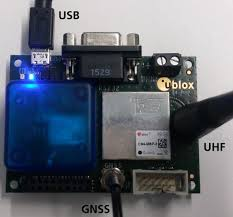
\includegraphics{img/montage.jpg}
    \caption{Photo du montage d'un module}
\end{figure}

\subsection{Configuration}

Les deux modules du kit C94-M8P sont identiques physiquement. Ils doivent être
configurés chacune leur tour en tant que base et rover respectivement. En
utilisant U-center, un seul module ne peut être configuré à la fois. Les
paramètres suggérés dans le guide UBlox \cite{WEB08} ne posent pas de problème
et semble êtres parfaitement adaptés.

Une fois les deux modules configurés, il suffit de les alimenter pour qu'ils
fonctionnent.  Afin de pouvoir apprécier les premiers résultats, on branche la
base et le rover à deux PC différents car U-center ne supporte qu'une seule
connexion USB simultanée.  Après que la phase d'initialisation soit terminée,
les modules sont prêts à fonctionner.

Pour que les modules utilisent le mode \gls{dgps}, la base doit définir sa
position précisément. Pour ce faire, deux modes sont disponibles:

\subsection{Survey-in}
Si on ne connaît pas la position GPS précise de la base, elle devra la calculer
elle même (\textit{Survey-in}). Cela consiste en un temps d'attente défini où
la base essaie de déduire sa position en partant du principe qu'elle est
immobile. Toute dérive de sa position est alors considérée comme une erreur
potentielle. Plus la base reste dans ce mode, plus elle peut déduire une
position précise. En rase campagne on peut ainsi espérer une précision
horizontale de 150 cm en 5 min, moins de 1 m au bout de plus d'une heure. Le
mode \textit{Survey-in} prend deux paramètres, le temps d'attente minimale et
la dérive horizontale visée. Ce mode s'arrête dès que ces deux paramètres sont
satisfaits. La base sera dés lors considérée comme fixe, et sa dérive
horizontale ne s'améliorera plus.

\subsection{Position connue}
Si on connaît la position de la base avec précision, par exemple à l'aide d'un
cadastre ou de références topographiques, on peut donner directement les
coordonnées GPS à la base et ainsi diviser le temps d'attente du mode
\textit{Survey-in}.


\subsection{Premiers résultats}
Pour nos premiers essais nous avons utilisé le mode \textit{Survey-in} pendant
300 sec et avec une précision horizontale minimale attendue de 150 cm. La base
était placée en haut d'un mat de 2 m au milieu d'un terrain dégagé sur
plusieurs centaines de mètres. Le mode \textit{Survey-in} n'a donc pas pris
plus de 5 minutes et la précision horizontale a pu tomber a 134 cm.

La base commence en mode 'TIME' ce qui signifie qu'elle communique en
\gls{rtcm} avec le rover mais que le mode \gls{dgps} ne fonctionne pas. En
effet malgré le fait que la base et le rover  communiquent, les données GPS
doivent êtres d'une qualité excellente avant que le mode \gls{dgps} puisse
fonctionner. Il faudra attendre plusieurs minutes encore avant que le rover et
la base se synchronisent et que la base passe finalement en mode 'FIXED'.

Le rover, quant à lui, commence en mode '3D/DGNSS' tant qu'il ne capte pas la
base ou que la base ne connaît pas encore sa position. Il passea ensuite au
mode '3D/DGNSS/FLOAT' lorsque la base est en mode 'TIME' et qu'elle lui
communique sa position via l'antenne UHF et enfin au mode '3D/DGNSS/FIXED'
lorsque le mode \gls{dgps} est fonctionnel.

Nous pouvons voir sur la photo ci-dessous la carte représentant la déviation de
la position obtenue en mode FIXED. On peut voir que l'échelle n'est que sur 10
cm et que la plus part des points sont dans un cercle représentant 5 cm. La
précision en mode FIXED est donc très impressionnante.

\begin{figure}[!htbp]
    \centering
	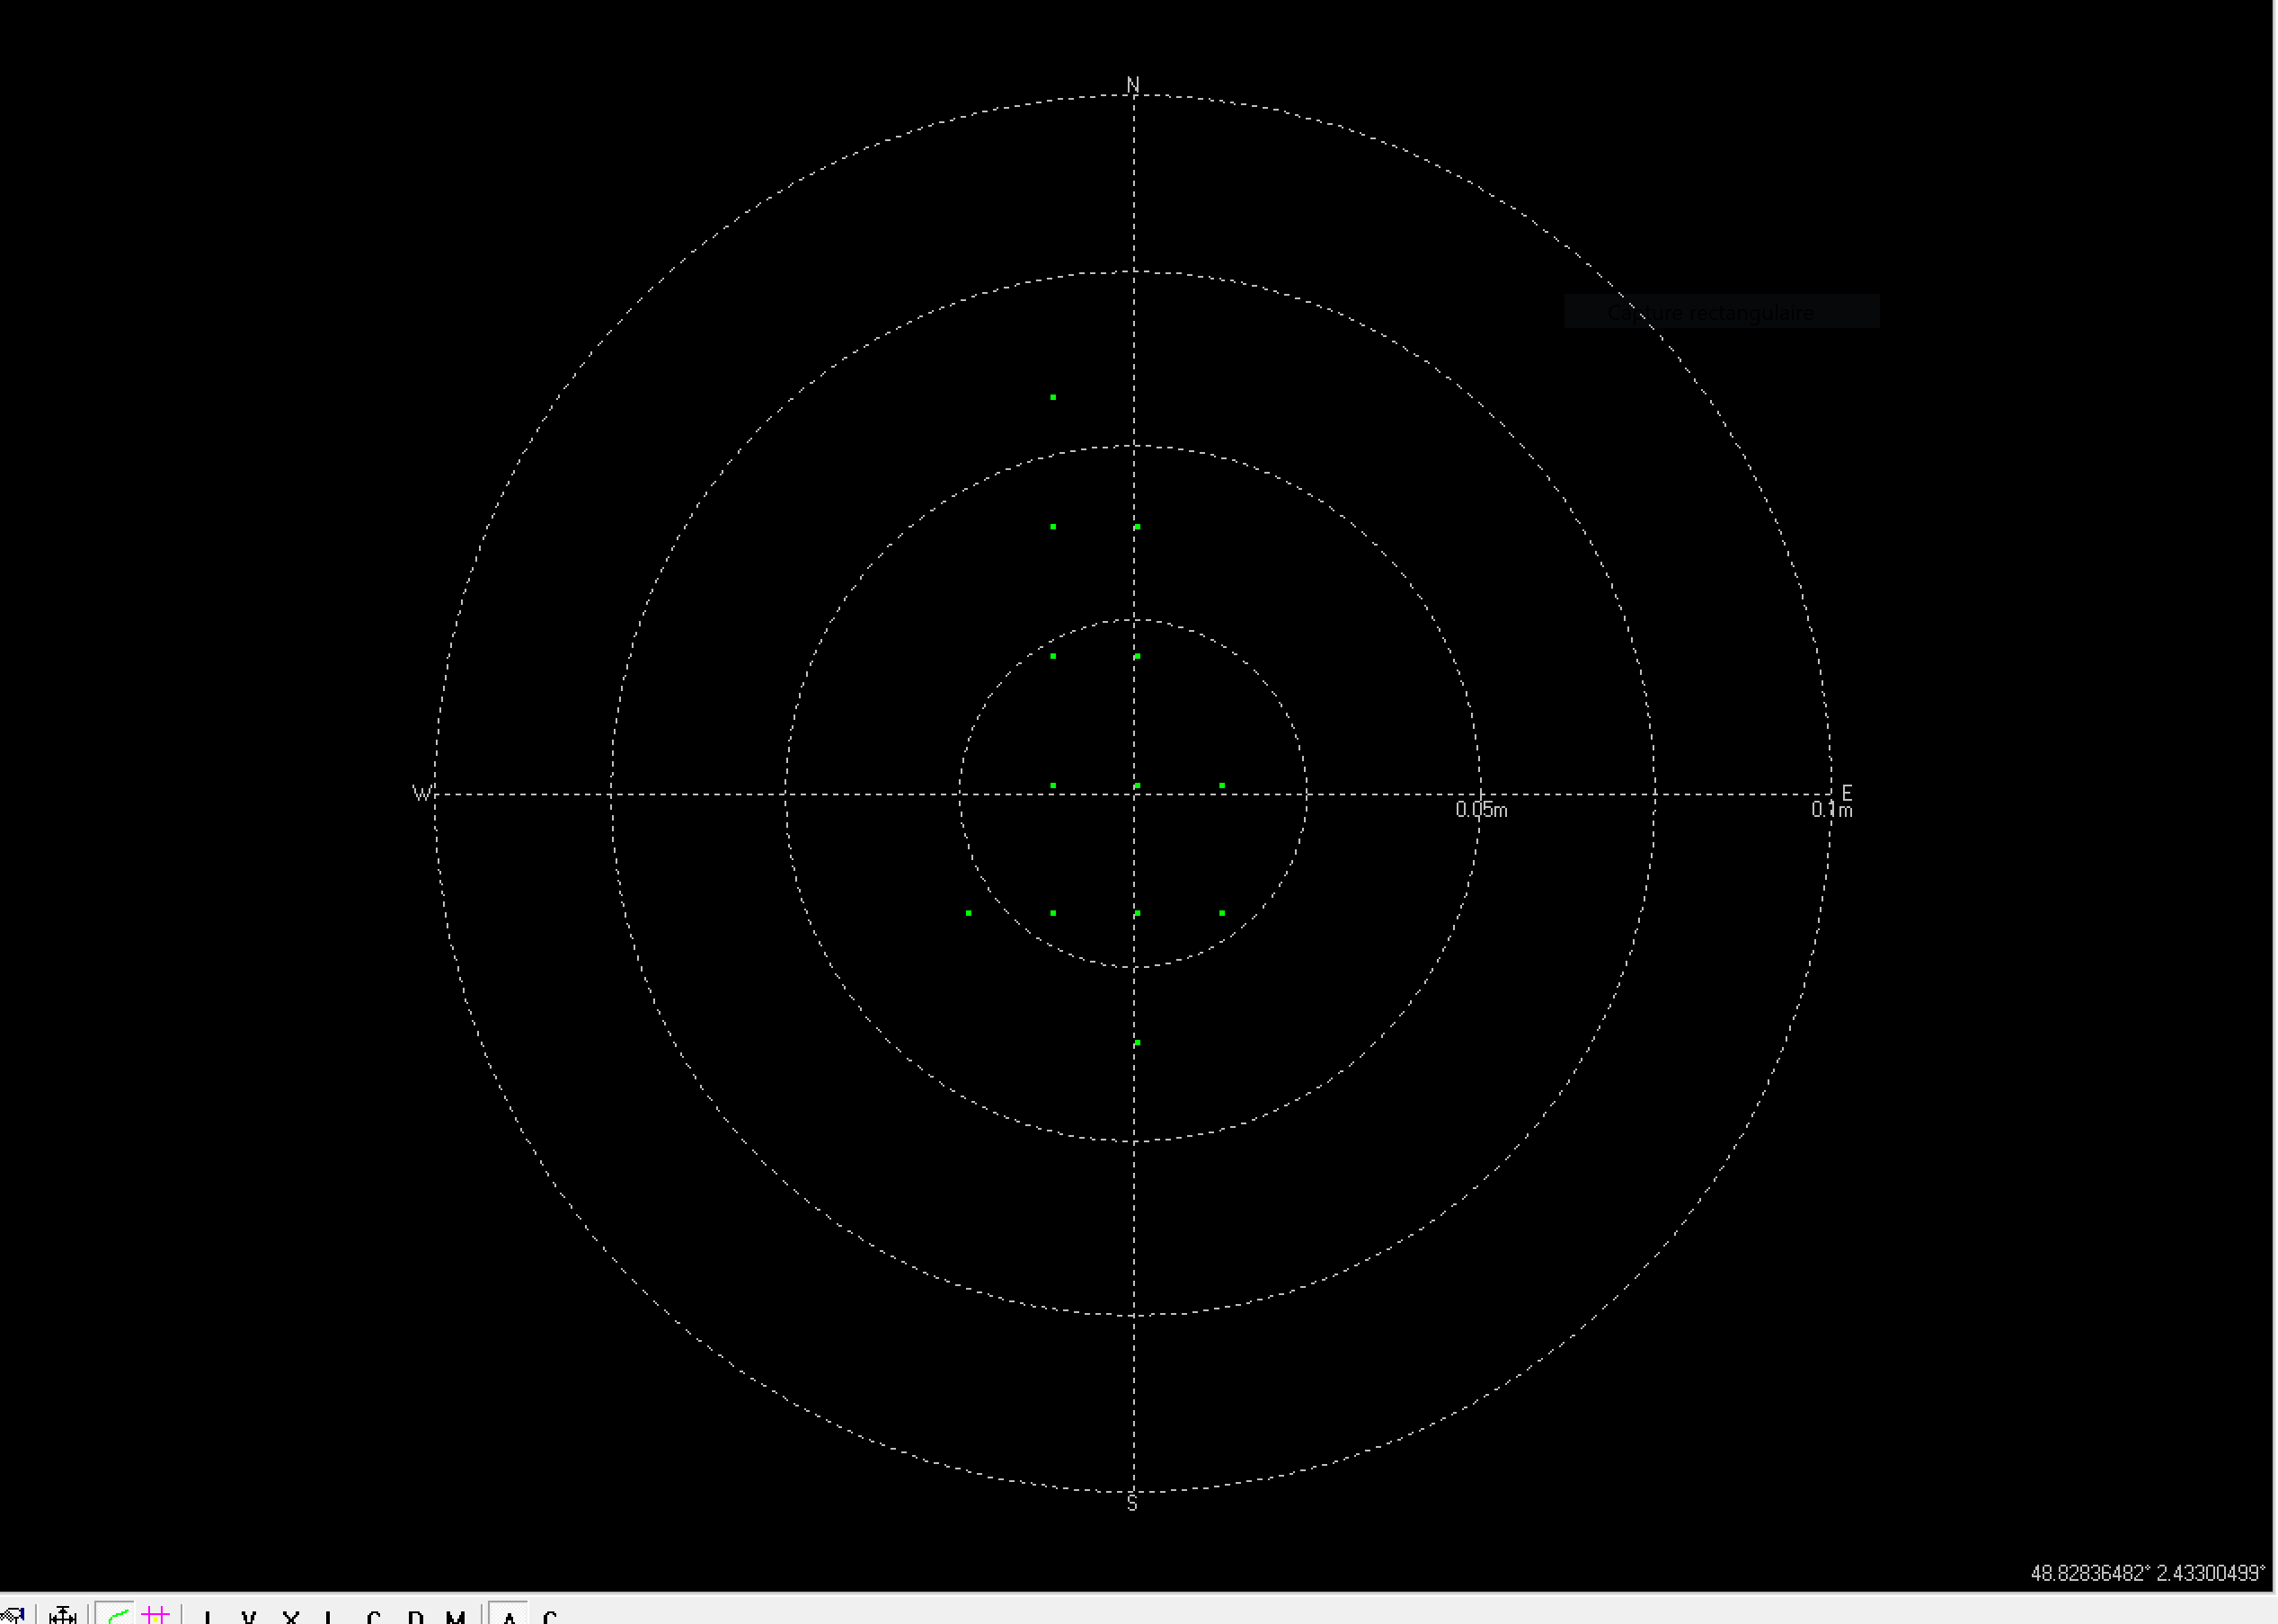
\includegraphics[width=\textwidth]{img/deviation.PNG}
    \caption{Photo de la déviation map avec comme }
\end{figure}









%-----------------------
\chapter{ROS}
%-----------------------

Pour récupérer les informations des modules \gls{gnss}, nous allons utiliser \acrfull{ros}. Les tests et les commandes montrés ici ont été réalisés avec \textit{l'interlogiciel} ROS-lunar tournant sur Arch Linux mais devraient marcher avec toutes les autres distributions linux compatibles avec \gls{ros}.

%-----------------------
\section{Démarrage rapide}
%-----------------------

Nous allons utiliser le package "Ublox" (http://wiki.ros.org/ublox). Afin de se servir d'un package \gls{ros} nous avons besoin de compiler les nœuds inhérents au package.Pour ce faire nous devons configurer un environnement catkin (le \textit{build system} spécialement fait pour \gls{ros} qui hérite de CMake.

Pour ce faire, il faut choisir un dossier qui sera notre "catkin workspace".

\begin{lstlisting}[style=msgTerminal]
$ mkdir -p ~/catkin_ws/src && cd ~/catkin_ws
\end{lstlisting}

Catkin n'est pas compatible avec python3, si votre distribution linux utilise python3 par défaut il faut indiquer à catkin le path vers python2.

\begin{lstlisting}[style=msgTerminal]
$ catkin_make -DPYTHON_EXECUTABLE=/usr/bin/python2
\end{lstlisting}

Il vous faudra ensuite sourcer le script de configuration d’environnement généré qui correspond à votre shell (.zsh si vous utilisez zsh etc..).

\begin{lstlisting}[style=msgTerminal]
$ source ~/catkin_ws/devel/setup.bash
\end{lstlisting}

Une fois toutes ces étapes réalisées, nous allons maintenant compiler le nœud ROS depuis les sources.
\begin{lstlisting}[style=msgTerminal]
$ cd ~/catkin_ws/src
$ git clone https://github.com/KumarRobotics/ublox.git
$ cd ~/catkin_ws
$ catkin_make -DCMAKE_BUILD_TYPE=Release
$ source ~/ros_catkin_ws/devel/setup.bash
\end{lstlisting}

Une fois la compilation terminée nous pouvons lancer le nœud grâce à roslaunch.

Pour le rover :
\begin{lstlisting}[style=msgTerminal]
$ roslaunch ublox_gps ublox_device.launch param_file_name:=c94_m8p_rover node_name:=ublox_gps
\end{lstlisting}

Pour la base :
\begin{lstlisting}[style=msgTerminal]
$ roslaunch ublox_gps ublox_device.launch param_file_name:=c94_m8p_base node_name:=ublox_gps
\end{lstlisting}

Les paramètres de la commande ci-dessus correspondent à ceux requis par le fichier ublox\_device.launch,
Pour paramétrer les GPS, il convient de modifier les fichiers ~/catkin\_ws/src/ublox/ublox\_gps/config/c94\_m8p\_base.yaml et \\~/catkin\_ws/src/ublox/ublox\_gps/config/c94\_m8p\_rover.yaml

Il est par exemple paramétré pour la base d'être le device /dev/ttyACM0 et pour le rover /dev/ttyACM1.

%-----------------------
\section{Récupérer les informations}
%-----------------------

Après connexion des deux modules, on peut commencer à lire les informations envoyées par ceux-ci. Le n\oe{}casse toiud ublox nous permet d'avoir plusieurs niveaux de verbosité (de 0 à 4 avec 0 pour 0 message de debug et 4 pour l'affichage de l'intégralité du contenu des trames). Pour choisir cela on modifie le champ "debug" du fichier "config.yaml".

\begin{figure}[!htbp]
\begin{center}
	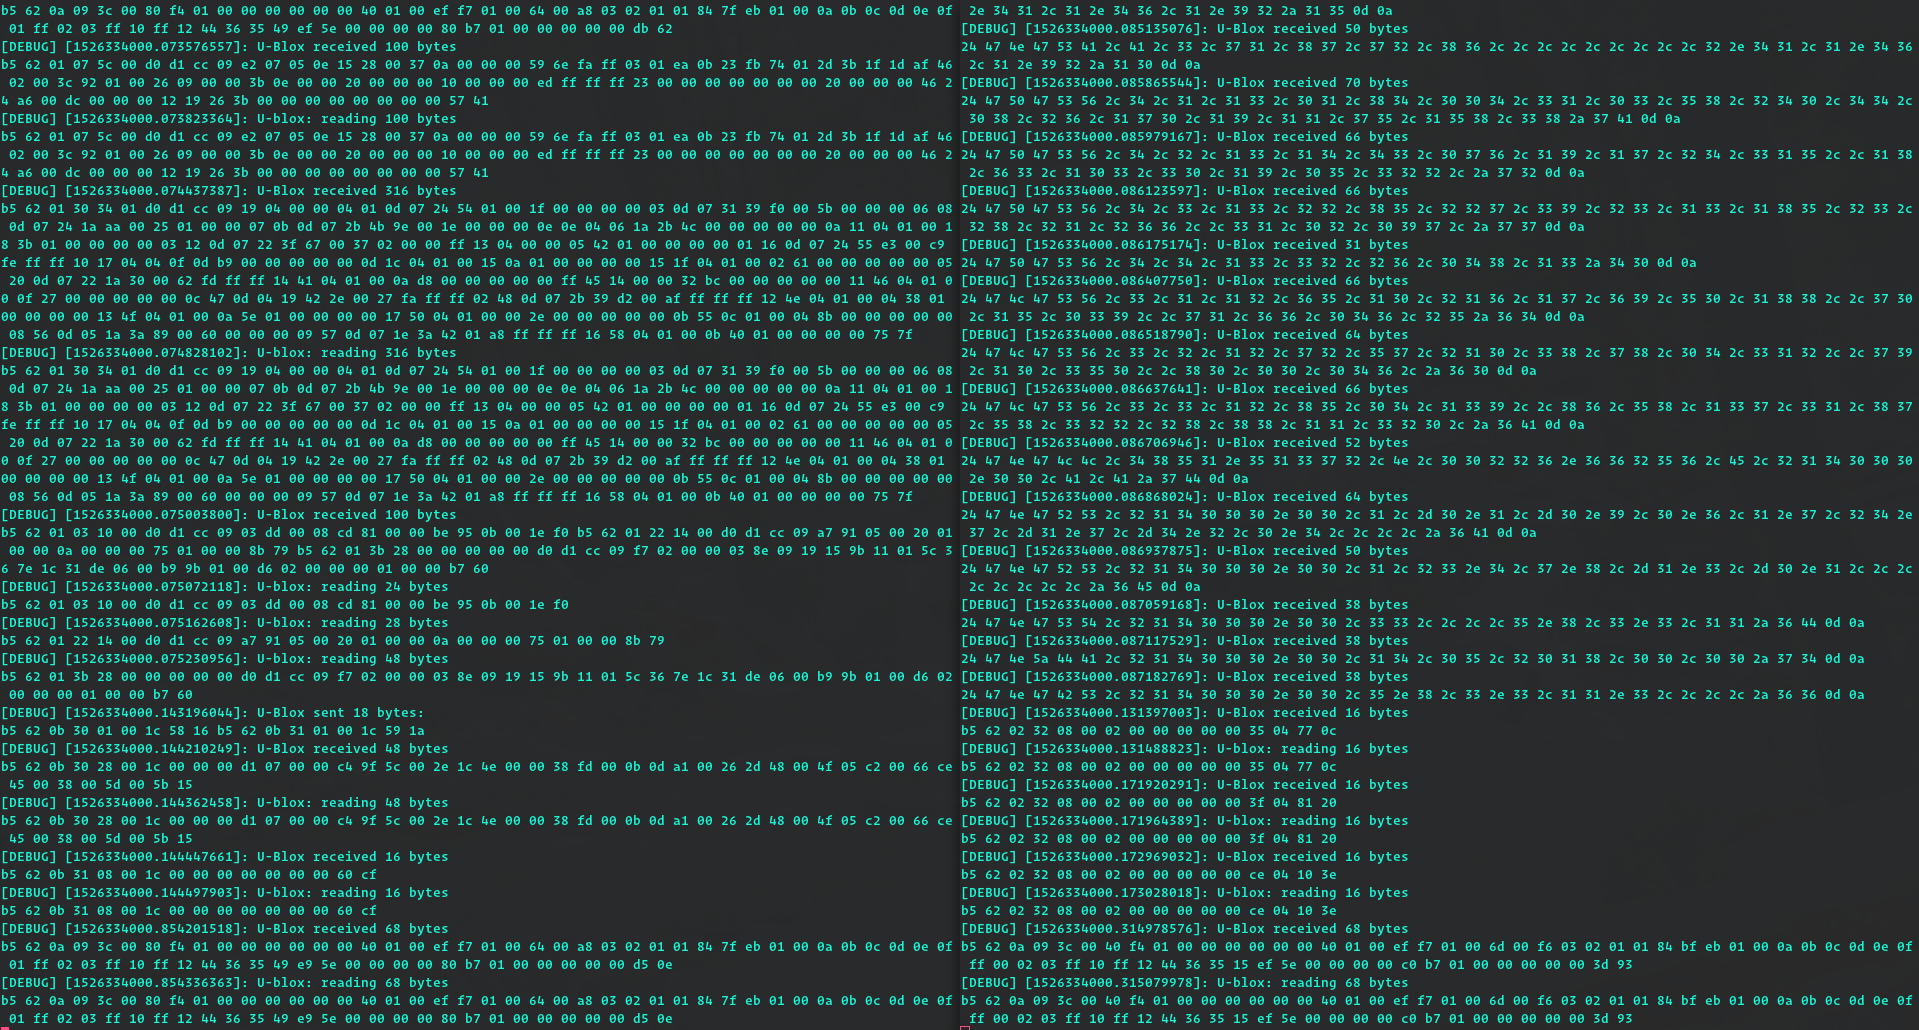
\includegraphics[width=\textwidth]{img/ros_node.png}
\end{center}
    \caption{Une fois les deux devices branchés (mode debug 4)}
\end{figure}

Il s'agit ensuite de récupérer les informations qui vont être postées sur des "forums" par le noeud ublox. Pour cela nous allons nous-mêmes créer notre noeud ROS qui va "subscribe" au bon topic sur le forum et traiter les données (pour plus de précisions sur les termes entre guillemets se référer à \cite{NOM06}).

Nous allons pour cela écrire un simple script python qui va afficher chaque position reçue sur un graphe grace à la librairie pyplot.
\vspace{3cm}
%-----------------------
\subsection{Script python d'affichage de position}
%-----------------------

Après avoir importé rospy (la librairie python officielle de ros) en haut de notre script, nous allons écrire une fonction d'initialisation.
\vspace{0.5cm}
\begin{python}
def init_subscriber():

  rospy.init_node('ublox_plot')
  rospy.Subscriber('ublox_gps_rover/fix', NavSatFix, loggpsdata)
  rospy.spin()

\end{python}

\vspace{0.5cm}
Ligne 3 on initialise un nouveau noeud ros qu'on appelle 'ublox\_plot'.
On va ensuite s'abonner au topic 'fix' du forum 'ublox\_gps\_rover'. La fonction Subscriber prend en argument 3 paramètres : le nom du forum/topic auquel l'on souhaite s'abonner, l'unité des données qui seront publiées sur ce forum et enfin une fonction callback (loggpsdata) que nous allons nous-même coder et qui sera appelée avec chaque nouveaux posts comme argument.
Enfin la fonction spin ligne 5 va empêcher python de quitter tant que le noeud est actif.
\vspace{0.5cm}
\begin{python}
def loggpsdata(data):

    global init
    rospy.loginfo("lat %s", data.latitude)
    rospy.loginfo("lon %s", data.longitude)
    if init == 0:
        plt.figure()
        plt.axis([ data.latitude - 0.0005, data.latitude + 0.00005,
            data.longitude - 0.00005, data.longitude + 0.00005])
        init = 1
    x.append(data.latitude)
    y.append(data.longitude)
    plt.scatter(data.latitude, data.longitude)
    plt.pause(0.2)
\end{python}

Grâce à la librairie matplotlib.pyplot que l'on importe, on va pouvoir afficher des points qui correspondent aux longitudes et latitudes des positions. Ceux-ci sont passés par l'objet 'data' qui a longitude et latitude pour attribut.

On a ensuite juste à appeler la fonction init\_subscriber depuis le main.

\begin{figure}[!htbp]
    \centering
	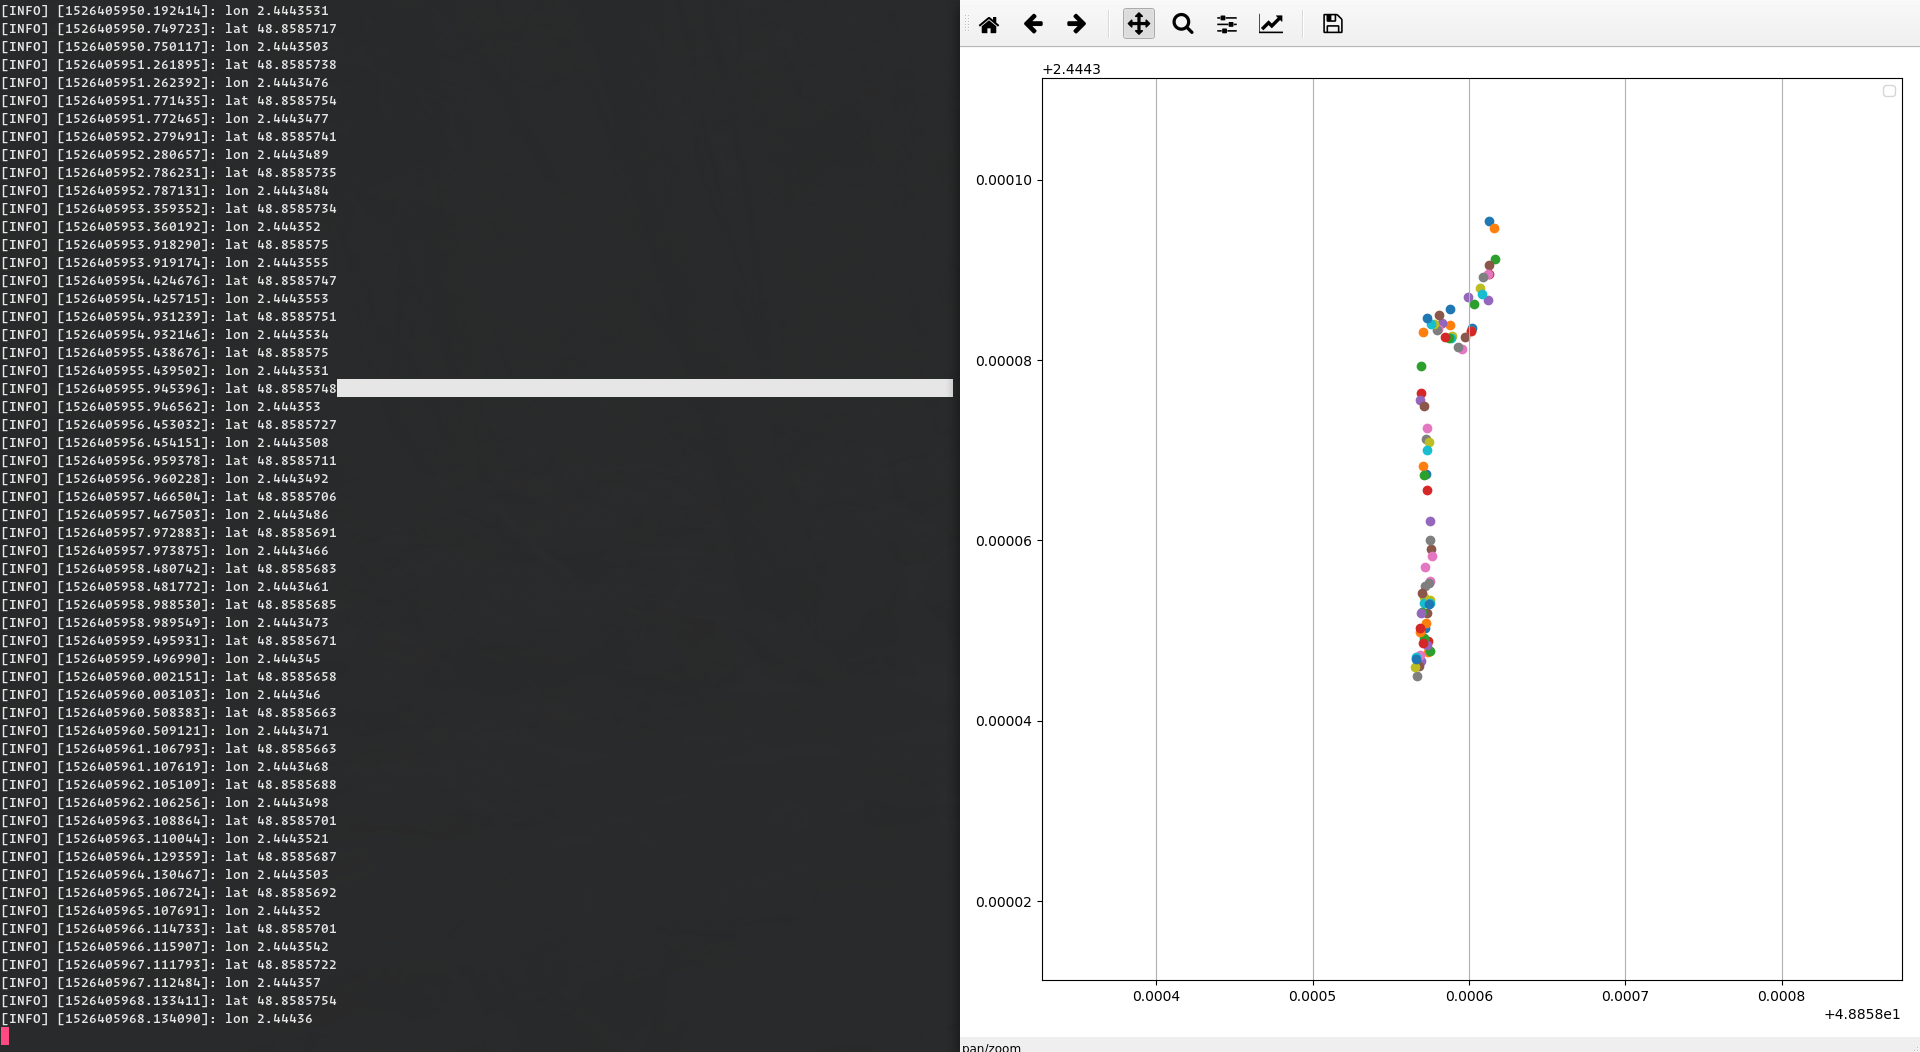
\includegraphics[width=\textwidth]{img/pyplot.png}
    \caption{Après avoir lancé le n\oe{}ud ublox pour les deux GPS puis lancé le noeud python ci-dessus}
\end{figure}
